\section*{Results}

\subsection*{Cisplatin and cyclophosphamide mutational signatures correlate with clinical treatment}

We identified mutational signatures for cisplatin, cyclophosphamide, and etoposide from the \textit{G. Gallus} cell line data (Figure~\ref{fig:supp_extracted_signatures_chicken}), as well as a second cisplatin signature from experiments in \textit{C. Elegans} (Figure~\ref{fig:supp_extracted_signatures_worm}). The two cisplatin signatures were not identical. Both signatures placed most probability mass on $C \rightarrow A$ mutations, but differed in preference for the nucleotides adjacent to the mutation. The \textit{G. Gallus} signature was relatively indifferent to the 5' base and favored a 3' cytosine, whereas the \textit{C. Elegans} signature was specific for a 5' cytosine and a 3' pyrmidine. The \textit{G. Gallus} cisplatin signature was closest in cosine distance to COSMIC \textit{Signature (24) Aflatoxin}, \textit{Signature (4) Smoking}, and \textit{Signature (29) Chewing tobacco}, all associated with guanine adducts. The \textit{C. Elegans} cisplatin signature was similar to \textit{Signature (4) Smoking}, \textit{Signature (20) Mismatch repair}, and \textit{Signature (14) Unknown}. The \textit{G. Gallus} cyclophosphamide signature favored $T \rightarrow A$ and $C \rightarrow T$ mutations and was most similar to COSMIC Signatures \textit{(25)}, \textit{(8)}, and \textit{(5)}, all of unknown etiology. The \textit{G. Gallus} etoposide signature distributed probability mass nearly uniformly across mutation contexts and was most similar to COSMIC \textit{Signature (5) Unknown}, \textit{Signature (3) BRCA}, and \textit{Signature (16) Unknown}. Overall, the chemotherapy signatures were no closer to any COSMIC signatures than the two most similar COSMIC signatures (\textit{Signature (12) Unknown} and \textit{Signature (26) Mismatch repair}) are to each other, suggesting that deconvolution could in principle distinguish their contributions.

We performed signature deconvolution on each sample's SNVs (top and middle of Figures~\ref{fig:supp_signatures} and ~\ref{fig:supplementary_signatures_no_cutofftop}). Detection of the cyclophosphamide signature at the 6\% threshold was associated with clinical cyclophosphamide treatment (Bonferroni-corrected Fischer's exact test $p = 0.004$), occurring in 4/10 samples taken after cyclophosphamide treatment, 2/79 pre-treatment samples, and 2/25 samples exposed to chemotherapies other than cyclophosphamide. In contrast, the two cisplatin signatures were found in no samples, and the etoposide signature was found only in four pre-treatment samples.

For better sensitivity, we next focused on the 14 relapse/treated samples from the 12 patients with both pre- and post-treatment samples. For each patient, we extracted the mutations that had evidence exclusively in the treated samples. Of 206,766 SNVs in the post-treatment samples for these patients, 93,986 (45\%) satisfied our filter and were subjected to signature deconvolution (Figure ~\ref{fig:signatures}, bottom of Figures~\ref{fig:supp_signatures} and ~\ref{fig:supplementary_signatures_no_cutofftop}). Within this subgroup, the \textit{G. gallus} cisplatin signature was identified only in the two samples taken after cisplatin therapy, a significant association ($p = 0.04$). The \textit{C. Elegans} cisplatin signature was detected in no samples, and the cyclophosphamide signature was detected in 3/6 cyclophosphamide-treated samples, but, unexpectedly, also in 6/8 non-cyclophosphamide-treated samples. These included the two post-treatment samples in which the signature was detected in the earlier analysis plus four additional samples. COSMIC \textit{Signature (3) BRCA} and \textit{Signature (8) Unknown etiology} were detected in 14/14 and 9/14 post-treatment samples, respectively, but \textit{Signature (1) Age} was absent, consistent with its association with a slow mutagenic process operative before oncogenesis.

In summary, the mutational signatures for cisplatin and cyclophosphamide extracted from experiments of a \textit{G. Gallus} cell line showed significant but inexact associations with clinical chemotherapy exposure.

\begin{figure}[htbp]
\centering
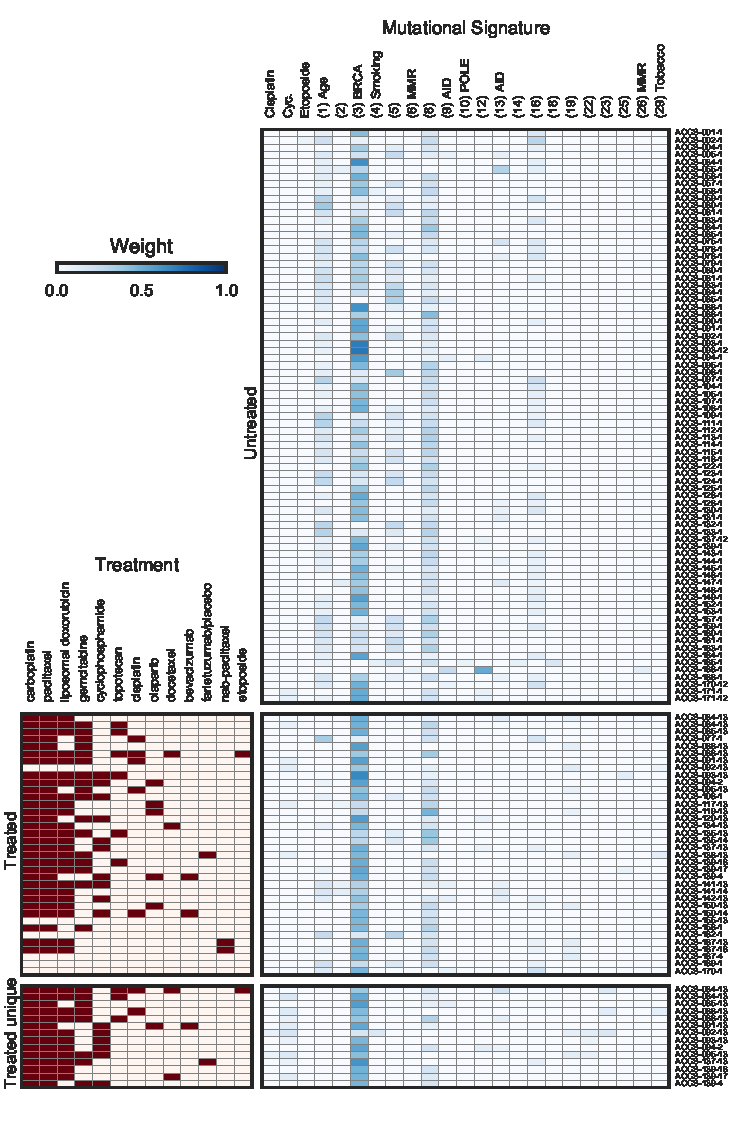
\includegraphics[scale=1.0]{figures/signatures.pdf}
\caption{\textbf{Detected mutational signatures for donor-matched primary/untreated and relapse/treated samples.} \textit{(Top)} Signatures detected in the pre-treatment samples. The first four signatures were extracted from reports of a \textit{G. gallus} cell line and \textit{C. Elegans} after exposure to chemotherapy, and the rest are COSMIC curated signatures. COSMIC signature numbers are shown in parentheses, and the associated mutagenic process is indicated when known. Signatures not shown were undetected in these samples. \textit{(Bottom)} Clinical treatments and detected signatures for the mutations unique to the post-treatment samples (those with no evidence in the matched pre-treatment sample). Cases where a chemotherapy signature is detected are annotated with a (*) if the patient received the associated drug and a (?) otherwise.}
\label{fig:signatures}
\end{figure}

\subsection*{Neoantigen burden increases at relapse}

% STATEMENT_TREATMENT_EFFECT
Across the cohort, we identified 17,689 mutated peptides predicted to bind autologous MHC class I with affinity 500nm or tighter ~\cite{Sette1994}. All but 21 (0.12\%) of these predicted neoantigens were private to a single patient (shared neoantigens are listed in Additional File 6).

Relapse/treated samples showed more expressed neoantigens than primary/untreated samples. Solid tissue relapse samples harbored a median of 81\% (bootstrap 95\% CI 40--123) more mutations, 124\% (58--191) more neoantigens, and 90\% (40--142) more expressed neoantigens than primary/untreated solid tissue samples (Figure~\ref{fig:counts}), all significant increases (Mann-Whitney $p < 0.004$ for each of the three tests). A similar trend was observed for ascites samples. Relapse/treated ascites samples harbored 31\% (14--49), 59\% (14--124), and 90\% (27--190) more mutations, neoantigens, and expressed neoantigens than primary/untreated ascites samples, respectively ($p=0.08, 0.11, 0.04$ for the three tests). This trend was also apparent in a comparison of paired samples from the same donors (Figure~\ref{fig:supp_paired}). 

In contrast, primary/treated samples, which were exposed to neoadjuvant chemotherapy (NACT) prior to surgery, did not exhibit increased numbers of mutations, neoantigens, or expressed neoantigens, and in fact trended toward decreased expressed neoantigen burden. The five primary/treated samples, all from solid tissue resections, harbored a median of 16 (9--89) expressed neoantigens compared to the median of 44 (39--60) observed in primary/untreated solid tissue samples, due to both fewer neoantigens in the DNA (median of 85 (36--306) vs. 130 (108--150)) and a lower rate of expression (median 19 (14--37) vs. 39 (36--42) percent of neoantigens). This trend did not reach significance (Mann-Whitney $p=0.09$), and will require larger cohorts to assess.

\begin{figure}
\centering
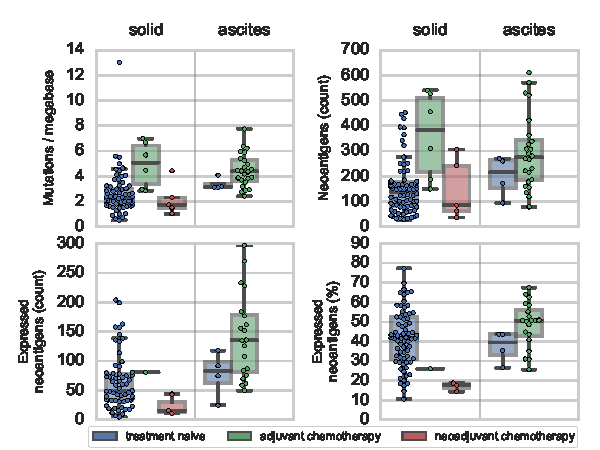
\includegraphics[scale=1.0]{figures/counts.pdf}
\caption{\textbf{Stratified comparison of mutation and neoantigen burden of chemotherapy-treated and untreated samples.} Mutations (upper left), neoantigens (upper right), and expressed neoantigens by count (lower left) and as a percent of total neoantigens (lower right) are shown for primary/untreated samples (blue; solid tumor n=75, ascites n=4), primary/treated samples (green; solid tumor n=5), and relapse/treated samples (red; solid tumor n=6, ascites n=24). The shaded boxes indicate the interquartile region and the median line. Points indicate individual samples.}
\label{fig:counts}
\end{figure}

\subsection*{Chemotherapy signatures weakly contribute to neoantigen burden at relapse}

%We next performed signature deconvolution on the mutations detected in each sample (Figure~\ref{fig:supp_signatures} top and middle).

While we cannot determine with certainty whether any particular mutation was chemotherapy-induced, we can estimate the fraction of mutations and neoantigens attributable to each signature in a sample (Figures~\ref{fig:sources} and~\ref{fig:sourcesungrouped}).

Similarly to results reported by Patch et al., the most prevalent mutational signatures in this cohort were COSMIC \textit{Signature (3)}, associated with BRCA disruption, \textit{Signature (8)}, of unknown etiology, and \textit{Signature (1)}, associated with spontaneous deamination of 5-methylcytosine, a slow process active in healthy tissue that correlates with age (Figure~\ref{fig:supp_signatures} top and middle). These signatures together accounted for a median of 67\% (95\% CI 66 - 69) of mutations, 58\% (56--61) of neoantigens, and 68\% (67--71) expressed neoantigens across samples. These rates did not substantially differ with chemotherapy treatment.

The chemotherapy signatures accounted for a small but detectable part of the increased neoantigen burden of relapse samples. In primary/untreated samples, which indicate the background rate of chance attribution, chemotherapy mutational signatures accounted for a mean of 2\% of the mutations (range 0--8), 2\% (0--7) of the neoantigens, and 2\% (0--8) of the expressed neoantigens. In each of the five primary/treated samples, less than 1\% of the mutation, neoantigen, and expressed neoantigen burdens were attributed to chemotherapy signatures. For the relapse/treated samples, chemotherapy signatures accounted for a mean of 6\% (range 0--21) of the mutations, 5\% (0--15) of the neoantigens, and 5\% (0--16) of the expressed neoantigens. The highest attribution to chemotherapy signatures occurred in sample AOCS-092-3-3, a relapse/treated sample from a patient who received five lines of platinum chemotherapy and eight distinct chemotherapeutic agents, the most in the cohort. For this sample, 21\% (or approximately 3,200 of 15,491) of the SNVs, 15\% (9 of 61) of the neoantigens, and 16\% (5 of 30) of the expressed neoantigens were attributed to chemotherapy signatures.

Signature deconvolution considers only SNVs, but studies of platinum-induced mutations have also reported increases in the rate of dinucleotide variants and indels. Indeed, we observed more MNVs overall and specifically the platinum-associated MNVs $CT \rightarrow AC$ and $CA \rightarrow AC$ reported by Meier et al.~\cite{Meier_2014} in treated patients in both absolute count and as a fraction of mutational burden ($p < 10^{-6}$ for all tests). Sample AOCS-092-3-3, previously found to have the most chemotherapy-signature SNVs, also had the most platinum-associated dinucleotide variants and the second-most MNVs overall. This sample harbored 59 $CT \rightarrow AC$ or $CA \rightarrow AC$ mutations, compared to a mean of 3.2 (2.2--4.4) across all samples. Treated samples also harbored more indels in terms of absolute count ($p=10^{-4}$). Overall, while MNVs and indels generate more neoantigens per mutation than SNVs, they are rare, comprising less than 3\% of the mutational burden and 13\% of the neantigens in every sample (Figure~\ref{fig:sources}), making it unlikely that chemotherapy-induced MNVs and indels have a large impact on neoantigen burden.

% It was recently reported that high variant-allele frequency (i.e. clonal) neoantigens are required to elicit a cytotoxic T cell response~\cite{McGranahan_2016}. In our study, in the treated samples, chemotherapy-associated SNVs had on average 11\% (8--15) lower variant allele frequency than other SNVs and were approximately half as likely to be found in the top decile of variant allele frequency.
% STATEMENT_UNIQUE_TO_TREATED_COUNT

\begin{figure}[htbp]
\centering
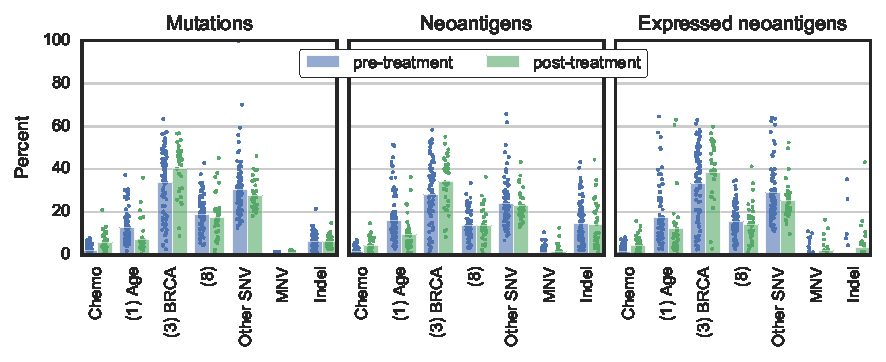
\includegraphics[scale=1.0]{figures/sources_of_mutations_and_neoantigens.pdf}
\caption{\textbf{Contribution of key SNV signatures, MNVs, and indels on mutations \textit{(left)}, neoantigens \textit{(center)}, and expressed neoantigens \textit{(right)}.} The \textit{Chemo} category combines the contributions from the chemotherapy signatures (cisplatin, cyclophosphamide, and etoposide). COSMIC signature numbers are in parentheses. The \textit{Other SNV} category represents SNVs not accounted for by the signatures shown. Bars give the mean, and points indicate individual samples.}
\label{fig:sources}
\end{figure}
